\documentclass[10pt]{beamer}

% \usepackage{define}
\usepackage{animate}

\usetheme{CCFD}
\usepackage{color}
\definecolor{gray97}{gray}{.90}
\definecolor{gray75}{gray}{.75}
\usepackage{listings}
\lstset{frame=Ltb,
     framerule=0pt,
     aboveskip=0cm,
     framextopmargin=0pt,
     framexbottommargin=0pt,
     framexleftmargin=0cm,
     framesep=0pt,
     rulesep=0pt,
     backgroundcolor=\color{gray97},
     rulesepcolor=\color{black},
     language=C,
           basicstyle=\ttfamily\scriptsize,
           keywordstyle=\color{blue}\ttfamily,
           stringstyle=\color{red}\ttfamily,
           commentstyle=\color{green}\ttfamily,
          breaklines=true,
          }
\lstdefinestyle{consol}
   {basicstyle=\scriptsize\bf\ttfamily,
    backgroundcolor=\color{gray75},
}
\resetcounteronoverlays{lstnumber}

\newcommand{\tabitem}{%
  \usebeamertemplate{itemize item}\hspace*{\labelsep}}

\usepackage{tikz}
\usetikzlibrary{calc,shapes,arrows.meta}

\eventtitle{Computer Science I}
\title{Lecture 10\\Dynamic memory allocation for 2D arrays\\{\tiny and examples}}
\date{}

\setbeamertemplate{blocks}[rounded][shadow=true]
\setbeamertemplate{navigation symbols}[]

\begin{document}

\frame{
    \titlepage
}

\section{Dynamic memory allocation}

\begin{frame}[fragile]
  \frametitle{Dynamic memory allocation}
  \framesubtitle{recall}  
\centering

\begin{lstlisting}
#include <stdlib.h>

void* malloc (unsigned int size);
\end{lstlisting}

\begin{enumerate}
	\item Allocates a block of \textbf{\textit{size}} bytes of memory
	\item Returns a pointer to the beginning of that block
	\item The content allocated block of memory is not initialized
	\item \textit{size t} is \textit{unsigned int}
	\item For each malloc there needs to be a single \textit{free}
\begin{lstlisting}
type * p = (type*)malloc(size);
free(p)
\end{lstlisting}
	\item \textbf{After} we are done with using the memory
\end{enumerate}
\end{frame}

\begin{frame}[fragile]
  \frametitle{Dynamic memory allocation}
  \framesubtitle{example}  
\centering
Read the size from keyboard and allocate memory to store doubles.

\begin{lstlisting}
#include <stdio.h>
#include <stdlib.h>

int mian(){
	int n;
	scanf("%d", &n);
	double *w = (double*)malloc(n*sizeof(double));
	free(w);
}
\end{lstlisting}

This is a 1D array, how about 2D?

\end{frame}
\begin{frame}[fragile]
  \frametitle{2D arrays}
  \framesubtitle{Recall the static 2D}
  \vspace{-0.3cm}
  \begin{columns}
    \begin{column}{0.65\textwidth}
      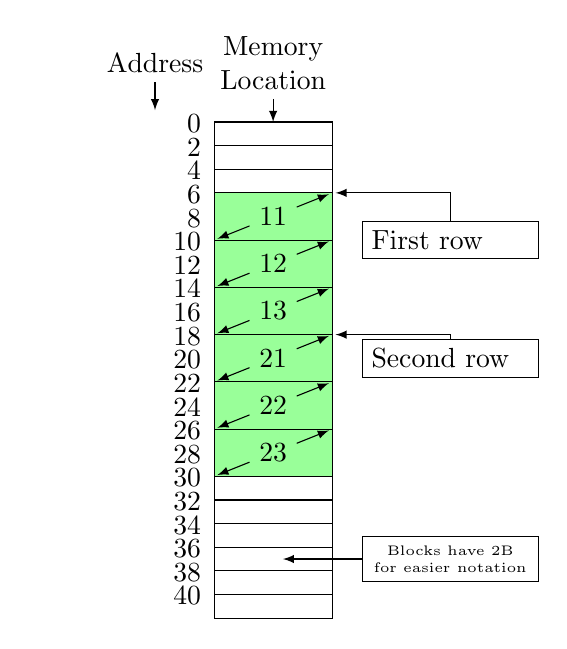
\begin{tikzpicture}[x=1.5cm,y=0.3cm]
  %% Building the boxes representing memory locations
  \foreach \x in {0,1,...,20}
  {
    \node[inner sep=1pt] (BL\x) at (0,-\x)   {};
    \node[inner sep=1pt] (UR\x) at (1,-\x+1) {};
    \node (MM\x) at ($(BL\x)!0.5!(UR\x)$) {};
    \draw (BL\x) rectangle (UR\x);
    \edef\memoryNumber{\number\numexpr0+2*\x}
    \node[anchor=south east] at (BL\x.north west) {\memoryNumber};
  }

  %% Label columns:
  \node (MEMLOC) at ($(MM0)+(0.0,0.9cm)$) { \parbox{2cm}{\centering Memory Location} };
  \node (ADDRESS) at ($(MEMLOC)-(1.0,0)$) {\parbox{3cm}{\centering Address} };
  \draw [-latex] (MEMLOC) -- ($(MM0|-UR0)+(0.0,0)$);
  \draw [-latex] (ADDRESS) -- ($(MM0|-UR0)-(1,-0.5)$);

  \foreach \x/\y in {4/3}
  {
    \draw[fill=green!40] (BL\x) rectangle (UR\y);
    \node (M\x-\y) at ($(BL\x)!0.5!(UR\y)$) {11};
    \draw[-latex]  (M\x-\y) -- (BL\x) ;
    \draw[-latex]  (M\x-\y) -- (UR\y) ;
  }
  \foreach \x/\y in {6/5}
  {
    \draw[fill=green!40] (BL\x) rectangle (UR\y);
    \node (M\x-\y) at ($(BL\x)!0.5!(UR\y)$) {12};
    \draw[-latex]  (M\x-\y) -- (BL\x) ; 
    \draw[-latex]  (M\x-\y) -- (UR\y) ;
  }
  \foreach \x/\y in {8/7}
  {
    \draw[fill=green!40] (BL\x) rectangle (UR\y);
    \node (M\x-\y) at ($(BL\x)!0.5!(UR\y)$) {13};
    \draw[-latex]  (M\x-\y) -- (BL\x) ; 
    \draw[-latex]  (M\x-\y) -- (UR\y) ;
  }
  \foreach \x/\y in {10/9}
  {
    \draw[fill=green!40] (BL\x) rectangle (UR\y);
    \node (M\x-\y) at ($(BL\x)!0.5!(UR\y)$) {21};
    \draw[-latex]  (M\x-\y) -- (BL\x) ; 
    \draw[-latex]  (M\x-\y) -- (UR\y) ;
  }
  \foreach \x/\y in {12/11}
  {
    \draw[fill=green!40] (BL\x) rectangle (UR\y);
    \node (M\x-\y) at ($(BL\x)!0.5!(UR\y)$) {22};
    \draw[-latex]  (M\x-\y) -- (BL\x) ; 
    \draw[-latex]  (M\x-\y) -- (UR\y) ;
  }
  \foreach \x/\y in {14/13}
  {
    \draw[fill=green!40] (BL\x) rectangle (UR\y);
    \node (M\x-\y) at ($(BL\x)!0.5!(UR\y)$) {23};
    \draw[-latex]  (M\x-\y) -- (BL\x) ; 
    \draw[-latex]  (M\x-\y) -- (UR\y) ;
  }
  
  \foreach \x/\y in {15/3}
  {
    \node[draw] (M\x-\y) at ($0.5*(UR\x)+0.5*(UR\y)+(1,4)$)
    { \parbox{2cm}{First row}};
    \draw[-latex]  (M\x-\y) |- (UR\y) ;
  }

  \foreach \x/\y in {19/9}
  {
    \node[draw] (M\x-\y) at ($0.5*(UR\x)+0.5*(UR\y)+(1,4)$)
    { \parbox{2cm}{Second row}};
    \draw[-latex]  (M\x-\y) |- (UR\y) ;
  }

    \node[draw] (M18) at ($(MM18)+(1.5,0)$)
    { \parbox{2cm}{\centering \tiny Blocks have 2B\\for easier notation}};
    \draw[-latex]  (M18) -- (MM18) ; 

\end{tikzpicture}
    \end{column}
    \begin{column}{0.5\textwidth}
      \begin{itemize}
        \item Indexing is from 0 to size-1
        \item Storage is row based
        \item Array is stored row after row
      \end{itemize}
Example:
\begin{lstlisting}
int tab[2][3];

tab[0][0]=11;
tab[0][1]=12;
tab[0][2]=13;

tab[1][0]=21;
tab[1][1]=22;
tab[1][2]=23;
\end{lstlisting}
\centering   
\begin{tikzpicture}
    \matrix[matrix of nodes,nodes={draw}] {
      11 & 12 & 13 \\
      21 & 22 & 23 \\
    };
\end{tikzpicture}

    \end{column}
  \end{columns}
\end{frame}


\begin{frame}[fragile]
  \frametitle{2D arrays}
  \framesubtitle{}  
  \vspace{-0.3cm}
  \begin{columns}
    \begin{column}{0.65\textwidth}
      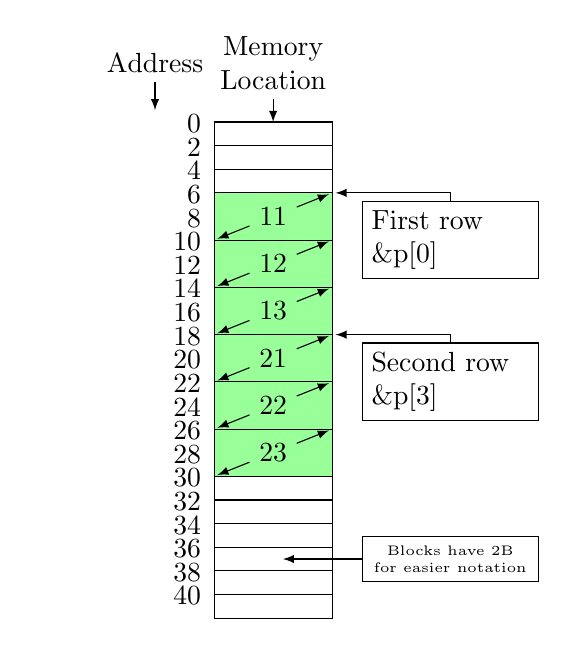
\begin{tikzpicture}[x=1.5cm,y=0.3cm]
  %% Building the boxes representing memory locations
  \foreach \x in {0,1,...,20}
  {
    \node[inner sep=1pt] (BL\x) at (0,-\x)   {};
    \node[inner sep=1pt] (UR\x) at (1,-\x+1) {};
    \node (MM\x) at ($(BL\x)!0.5!(UR\x)$) {};
    \draw (BL\x) rectangle (UR\x);
    \edef\memoryNumber{\number\numexpr0+2*\x}
    \node[anchor=south east] at (BL\x.north west) {\memoryNumber};
  }

  %% Label columns:
  \node (MEMLOC) at ($(MM0)+(0.0,0.9cm)$) { \parbox{2cm}{\centering Memory Location} };
  \node (ADDRESS) at ($(MEMLOC)-(1.0,0)$) {\parbox{3cm}{\centering Address} };
  \draw [-latex] (MEMLOC) -- ($(MM0|-UR0)+(0.0,0)$);
  \draw [-latex] (ADDRESS) -- ($(MM0|-UR0)-(1,-0.5)$);

  \foreach \x/\y in {4/3}
  {
    \draw[fill=green!40] (BL\x) rectangle (UR\y);
    \node (M\x-\y) at ($(BL\x)!0.5!(UR\y)$) {11};
    \draw[-latex]  (M\x-\y) -- (BL\x) ;
    \draw[-latex]  (M\x-\y) -- (UR\y) ;
  }
  \foreach \x/\y in {6/5}
  {
    \draw[fill=green!40] (BL\x) rectangle (UR\y);
    \node (M\x-\y) at ($(BL\x)!0.5!(UR\y)$) {12};
    \draw[-latex]  (M\x-\y) -- (BL\x) ; 
    \draw[-latex]  (M\x-\y) -- (UR\y) ;
  }
  \foreach \x/\y in {8/7}
  {
    \draw[fill=green!40] (BL\x) rectangle (UR\y);
    \node (M\x-\y) at ($(BL\x)!0.5!(UR\y)$) {13};
    \draw[-latex]  (M\x-\y) -- (BL\x) ; 
    \draw[-latex]  (M\x-\y) -- (UR\y) ;
  }
  \foreach \x/\y in {10/9}
  {
    \draw[fill=green!40] (BL\x) rectangle (UR\y);
    \node (M\x-\y) at ($(BL\x)!0.5!(UR\y)$) {21};
    \draw[-latex]  (M\x-\y) -- (BL\x) ; 
    \draw[-latex]  (M\x-\y) -- (UR\y) ;
  }
  \foreach \x/\y in {12/11}
  {
    \draw[fill=green!40] (BL\x) rectangle (UR\y);
    \node (M\x-\y) at ($(BL\x)!0.5!(UR\y)$) {22};
    \draw[-latex]  (M\x-\y) -- (BL\x) ; 
    \draw[-latex]  (M\x-\y) -- (UR\y) ;
  }
  \foreach \x/\y in {14/13}
  {
    \draw[fill=green!40] (BL\x) rectangle (UR\y);
    \node (M\x-\y) at ($(BL\x)!0.5!(UR\y)$) {23};
    \draw[-latex]  (M\x-\y) -- (BL\x) ; 
    \draw[-latex]  (M\x-\y) -- (UR\y) ;
  }
  
  
  \foreach \x/\y in {15/3}
  {
    \node[draw] (M\x-\y) at ($0.5*(UR\x)+0.5*(UR\y)+(1,4)$)
    { \parbox{2cm}{First row\\ \&p[0]}};
    \draw[-latex]  (M\x-\y) |- (UR\y) ;
  }

  \foreach \x/\y in {19/9}
  {
    \node[draw] (M\x-\y) at ($0.5*(UR\x)+0.5*(UR\y)+(1,3)$)
    { \parbox{2cm}{Second row\\ \&p[3]}};
    \draw[-latex]  (M\x-\y) |- (UR\y) ;
  }

    \node[draw] (M18) at ($(MM18)+(1.5,0)$)
    { \parbox{2cm}{\centering \tiny Blocks have 2B\\for easier notation}};
    \draw[-latex]  (M18) -- (MM18) ; 

\end{tikzpicture}
    \end{column}
    \begin{column}{0.55\textwidth}

\begin{lstlisting}
int *p=(int*)malloc(24);

p[0] = 11;
p[1] = 12;
p[2] = 13;
p[3] = 21;
p[4] = 22;
p[5] = 23;

free(p);
\end{lstlisting}

    \end{column}
  \end{columns}
\end{frame}

\begin{frame}[fragile]
  \frametitle{2D arrays}
  \framesubtitle{Pointers to pointers}  
  \vspace{-0.3cm}


\begin{lstlisting}
int a = 5;
int *p=&a;
int **pp=&p;// !!!

printf("%d", a);//simple
printf("%d", *p);//still simple
printf("%d", *(*pp));//?

...
printf("%d", a);//simple
printf("%d", p[0]);//still simple
printf("%d", pp[0][0]));//?

\end{lstlisting}

\end{frame}

\begin{frame}[fragile]
  \frametitle{2D arrays}
  \framesubtitle{}  
  \vspace{-0.3cm}
  \begin{columns}
    \begin{column}{0.65\textwidth}
      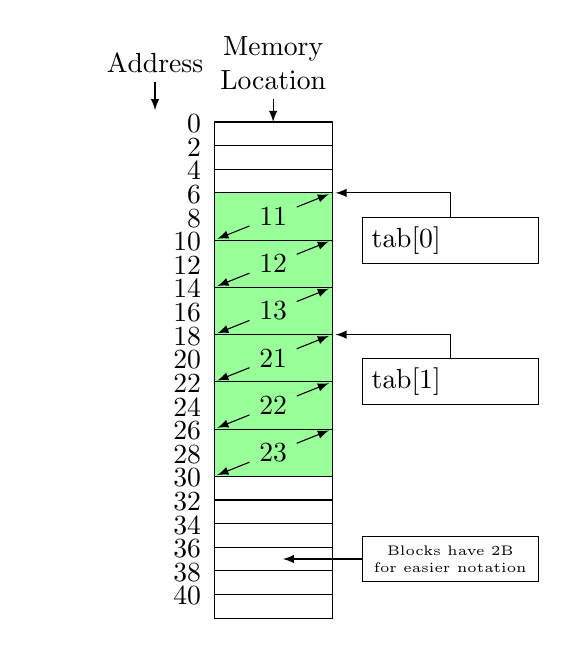
\begin{tikzpicture}[x=1.5cm,y=0.3cm]
  %% Building the boxes representing memory locations
  \foreach \x in {0,1,...,20}
  {
    \node[inner sep=1pt] (BL\x) at (0,-\x)   {};
    \node[inner sep=1pt] (UR\x) at (1,-\x+1) {};
    \node (MM\x) at ($(BL\x)!0.5!(UR\x)$) {};
    \draw (BL\x) rectangle (UR\x);
    \edef\memoryNumber{\number\numexpr0+2*\x}
    \node[anchor=south east] at (BL\x.north west) {\memoryNumber};
  }

  %% Label columns:
  \node (MEMLOC) at ($(MM0)+(0.0,0.9cm)$) { \parbox{2cm}{\centering Memory Location} };
  \node (ADDRESS) at ($(MEMLOC)-(1.0,0)$) {\parbox{3cm}{\centering Address} };
  \draw [-latex] (MEMLOC) -- ($(MM0|-UR0)+(0.0,0)$);
  \draw [-latex] (ADDRESS) -- ($(MM0|-UR0)-(1,-0.5)$);

  \foreach \x/\y in {4/3}
  {
    \draw[fill=green!40] (BL\x) rectangle (UR\y);
    \node (M\x-\y) at ($(BL\x)!0.5!(UR\y)$) {11};
    \draw[-latex]  (M\x-\y) -- (BL\x) ;
    \draw[-latex]  (M\x-\y) -- (UR\y) ;
  }
  \foreach \x/\y in {6/5}
  {
    \draw[fill=green!40] (BL\x) rectangle (UR\y);
    \node (M\x-\y) at ($(BL\x)!0.5!(UR\y)$) {12};
    \draw[-latex]  (M\x-\y) -- (BL\x) ; 
    \draw[-latex]  (M\x-\y) -- (UR\y) ;
  }
  \foreach \x/\y in {8/7}
  {
    \draw[fill=green!40] (BL\x) rectangle (UR\y);
    \node (M\x-\y) at ($(BL\x)!0.5!(UR\y)$) {13};
    \draw[-latex]  (M\x-\y) -- (BL\x) ; 
    \draw[-latex]  (M\x-\y) -- (UR\y) ;
  }
  \foreach \x/\y in {10/9}
  {
    \draw[fill=green!40] (BL\x) rectangle (UR\y);
    \node (M\x-\y) at ($(BL\x)!0.5!(UR\y)$) {21};
    \draw[-latex]  (M\x-\y) -- (BL\x) ; 
    \draw[-latex]  (M\x-\y) -- (UR\y) ;
  }
  \foreach \x/\y in {12/11}
  {
    \draw[fill=green!40] (BL\x) rectangle (UR\y);
    \node (M\x-\y) at ($(BL\x)!0.5!(UR\y)$) {22};
    \draw[-latex]  (M\x-\y) -- (BL\x) ; 
    \draw[-latex]  (M\x-\y) -- (UR\y) ;
  }
  \foreach \x/\y in {14/13}
  {
    \draw[fill=green!40] (BL\x) rectangle (UR\y);
    \node (M\x-\y) at ($(BL\x)!0.5!(UR\y)$) {23};
    \draw[-latex]  (M\x-\y) -- (BL\x) ; 
    \draw[-latex]  (M\x-\y) -- (UR\y) ;
  }
  
  
  \foreach \x/\y in {15/3}
  {
    \node[draw] (M\x-\y) at ($0.5*(UR\x)+0.5*(UR\y)+(1,4)$)
    { \parbox{2cm}{tab[0]}};
    \draw[-latex]  (M\x-\y) |- (UR\y) ;
  }

  \foreach \x/\y in {19/9}
  {
    \node[draw] (M\x-\y) at ($0.5*(UR\x)+0.5*(UR\y)+(1,3)$)
    { \parbox{2cm}{tab[1]}};
    \draw[-latex]  (M\x-\y) |- (UR\y) ;
  }

    \node[draw] (M18) at ($(MM18)+(1.5,0)$)
    { \parbox{2cm}{\centering \tiny Blocks have 2B\\for easier notation}};
    \draw[-latex]  (M18) -- (MM18) ; 

\end{tikzpicture}
    \end{column}
    \begin{column}{0.55\textwidth}

\begin{lstlisting}
int *tab[2];//what is tab?
int *p=(int*)malloc(24);

tab[0] = &p[0];//but also tab[0]=p;
p[0] = 11;
p[1] = 12;
p[2] = 13;
tab[1] = &p[3];//but also tab[1]=p+3;
p[3] = 21;
p[4] = 22;
p[5] = 23;

tab[0][0] = ?

free(p);
\end{lstlisting}

    \end{column}
  \end{columns}
\end{frame}

\begin{frame}[fragile]
  \frametitle{2D arrays}
  \framesubtitle{Pointers to pointers}  
  \vspace{-0.3cm}

\begin{lstlisting}
int **A = (int**)malloc(number_of_rows * szieof(int*));
\end{lstlisting}

1.
\begin{lstlisting}
for(int i=0; i<number_of_rows; ++i)
	A[i] = (int*)malloc(number_of_columns * sizeof(int));
\end{lstlisting}

2.
\begin{lstlisting}
int *p =(int*)malloc(collumns*rows*sizeof(int));
for(int i=0; i<number_of_rows; ++i)
	A[i] = p+i*number_of_collumns;
\end{lstlisting}

1.
\begin{lstlisting}
for(int i=0; i<number_of_rows; ++i)
	free(A[i]);
free(A);
\end{lstlisting}

2.
\begin{lstlisting}
free(p);
free(A);
\end{lstlisting}

Example...

\end{frame}


\end{document}
